
\chapter{Experimental Evaluation}

In this section we discuss our experimental evaluation.
First we describe the benchmarks with datasets used in the experiments.
Afterwards, we discuss our results concerning the instrumentations for profiling our work metric.
Finally we present the results of the online {\itercomp}.

We implemented the instrumentations in LLVM 4.0.
The target platform is a Linux-4.4.27 system with an Intel Core i7-4770 3.40GHz Skylake~CPU with 16~GiB RAM.

\section{Benchmarks}

%{\Itercomp} is essentially based on repeatedly trying out a large number of compiler optimisations until the best combination of compiler optimisations is found for a particular program.
%Our main goal is to speed up {\itercomp} while targeting optimal performance across large input datasets.

For the experimental evaluation we have used a subset of the \textit{KDataSets} benchmark suit, which is the same benchmark and dataset suit used by Chen~\etal~\cite{chen10,chen12a}.
The KDataSets contains 1000 different inputs for each one of its benchmark programs.
These benchmarks cover a broad spectrum of application scenarios, ranging from simple embedded signal-processing tasks to common mobile-phone and desktop tasks.
The different inputs try to capture distinct characteristics in terms of workload sizes and how these workloads exercise different control flow paths.
A summary of the benchmark and dataset suit is shown in Table~\ref{tab:kdatasets}.

\begin{table}[h]
\centering
\scalebox{.8}{
\begin{tabular}{|c|c|c|c|}
\hline
\textbf{Program} & \textbf{LOC}    & \textbf{Input file size}            & \textbf{Input description}              \\ \hline % Domain
qsort         & 154    & 32K-1.8M                   & 3D coordinates                 \\ \hline
jpeg\_d       & 13501  & 3.6K-1.5M                  & JPEG images                    \\ \hline
jpeg\_c       & 14014  & 16K-137M                   & PPM images                     \\ \hline
tiff2bw       & 15477  & \multirow{4}{*}{9K-137M}   & \multirow{4}{*}{TIFF images}   \\ \cline{1-2}
tiff2rgba     & 15424  &                            &                                \\ \cline{1-2}
tiffdither    & 15399  &                            &                                \\ \cline{1-2}
tiffmedian    & 15870  &                            &                                \\ \hline
susan\_c      & 1376   & \multirow{3}{*}{12K-46M}   & \multirow{3}{*}{PGM images}    \\ \cline{1-2}
susan\_e      & 1376   &                            &                                \\ \cline{1-2}
susan\_s      & 1376   &                            &                                \\ \hline
adpcm\_c      & 210    & 167K-36M                   & WAVE audios                    \\ \hline
adpcm\_d      & 211    & 21K-8.8M                   & ADPCM audios                   \\ \hline
lame          & 14491  & 167K-36M                   & WAVE audios                    \\ \hline
rsynth        & 4111   & 0.1K-42M                   &  Text files                    \\ \hline
sha           & 197    & 0.6K-35M                   & Files of any format            \\ \hline
\rowcolor{gray!20}
bitcount      & 460    &  -                         & Numbers: random                \\ \hline
\rowcolor{gray!20}
dijkstra      & 163    & 0.06K-4.3M                 & Adjacency matrices             \\ \hline
\rowcolor{gray!20}
patricia      & 290    & 0.6K-1.9M                  & IP and mask pairs              \\ \hline
\rowcolor{gray!20}
mad           & 2358   & 28K-27M                    & MP3 audios                     \\ \hline
\rowcolor{gray!20}
%gsm           & 3806   & 83K-18M                    & Sun/NeXT audios                \\ \hline
ghostscript   & 99869  & 11K-43M                    & Postscript files               \\ \hline
\rowcolor{gray!20}
%ispell        & 6522   & \multirow{3}{*}{0.1K-42M}  & \multirow{3}{*}{Text files}    \\ \cline{1-2}
%rsynth        & 4111   &                            &                                \\ \cline{1-2}
stringsearch  & 338    &  0.1K-42M                 &  Text files                     \\ \hline
\rowcolor{gray!20}
%blowfish\_e   & 863    & 0.6K-35M                   & Files of any format            \\ \hline
%blowfish\_d   & 863    & 0.6K-35M                   & Encrypted files                \\ \hline
%pgp\_e        & 19575  & 0.6K-35M                   & Files of any format            \\ \hline
%pgp\_d        & 19575  & 0.4K-18M                   & Encrypted files                \\ \hline
%rijndael\_e   & 952    & 0.6K-35M                   & Files of any format            \\ \hline
%rijndael\_d   & 952    & 0.7K-35M                   & Encrypted files                \\ \hline
CRC32         & 130    & 0.6K-35M                   & Files of any format            \\ \hline
\rowcolor{gray!20}
bzip2e        & 5125   & 0.7K-57M                   & Files of any format            \\ \hline
\rowcolor{gray!20}
bzip2d        & 5125   & 0.2K-25M                   & Compressed files               \\ \hline
\end{tabular}
}
\caption{Description of the KDataSets with 1000 inputs for each benchmark (Chen~\etal~\cite{chen10,chen12a}).}
\label{tab:kdatasets}
\end{table}

\section{Evaluation of the Instrumentation}

In this section we evaluate the performance of the work instrumentation presented in Chapter~\ref{chap:instr}, comparing between the optimal and the relaxed instrumentation with different thresholds.
%We organise the evaluation of the instrumentation as follows:

\subsection{Static Evaluation}

We first compare static aspects of the instrumentation algorithms.
The naive instrumentation always has 100\% of the basic blocks instrumented, by definition.
Figure~\ref{fig:num-probes} shows percentage of instrumented basic blocks for the optimal and the relaxed instrumentation with different relaxation thresholds.
While Figure~\ref{fig:num-probes} compares the different instrumentation algorithms in respect of the naive instrumentation, Figure~\ref{fig:num-probes-improvement} shows the improvement of the relaxation algorithm over the optimial instrumentation.

\begin{figure}[ht]
    \centering
    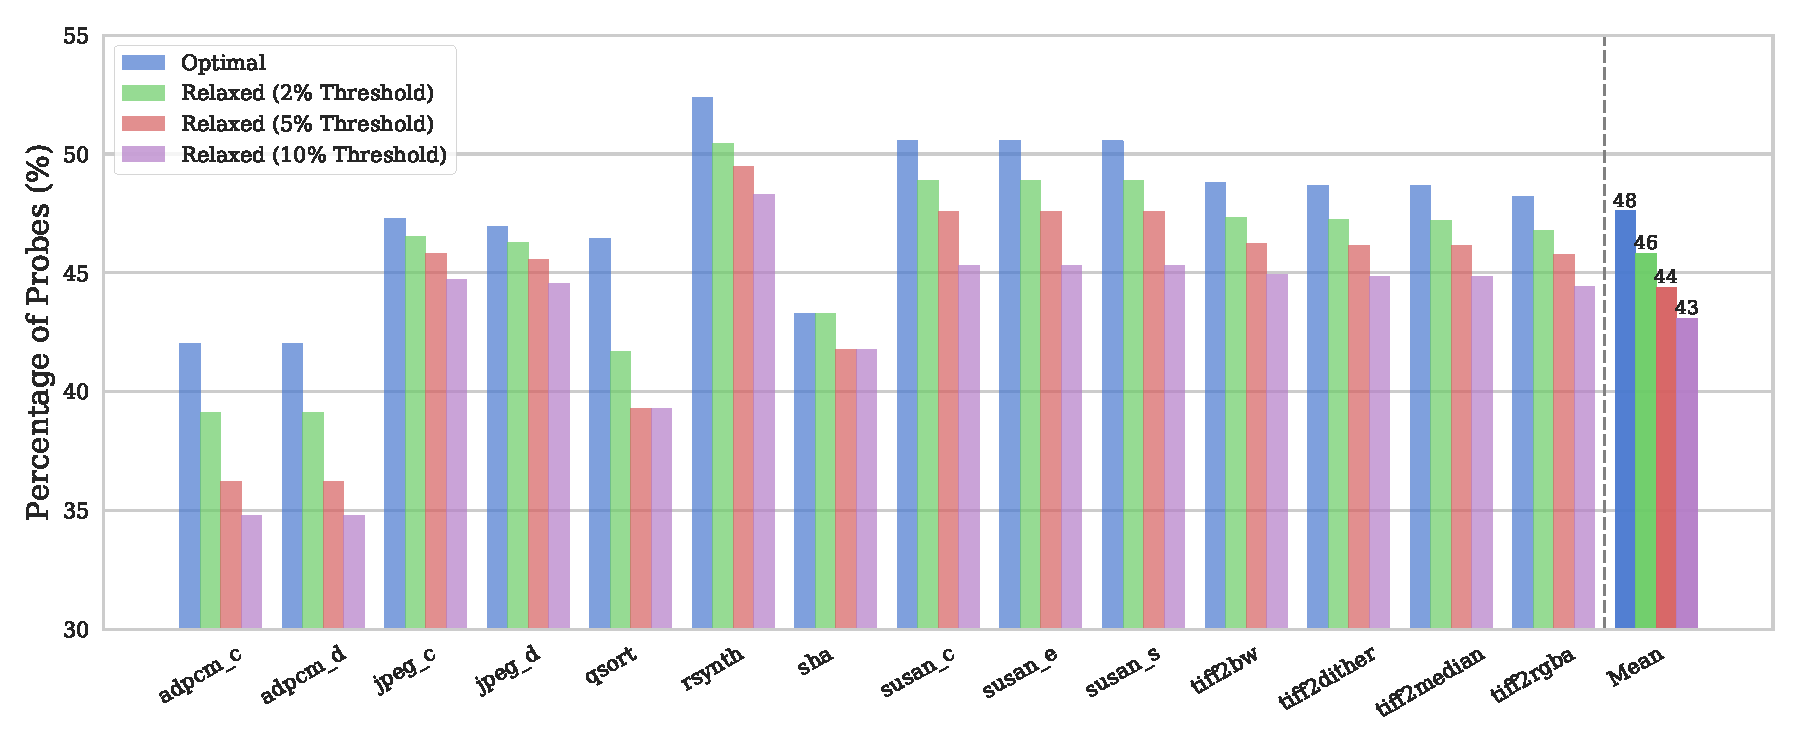
\includegraphics[width=\textwidth]{figs/num-probes.pdf}
    \caption{Percentage of instrumented basic blocks for the optimal and the relaxed instrumentation with different relaxation thresholds.}
    \label{fig:num-probes}
\end{figure}

Even a small threshold of 2\% is able to reduce the number of probes by an average of 5\% compared to the optimal algorithm. 
The \texttt{sha} benchmark was the only benchmark for which a 2\% threshold was not sufficient for further reducing the number of probes.
With a 10\% threshold the relaxation algorithm was able to improve over the optimal instrumentation by an average of 11\%, in terms of the amount of instrumented basic blocks.

\begin{figure}[ht]
    \centering
    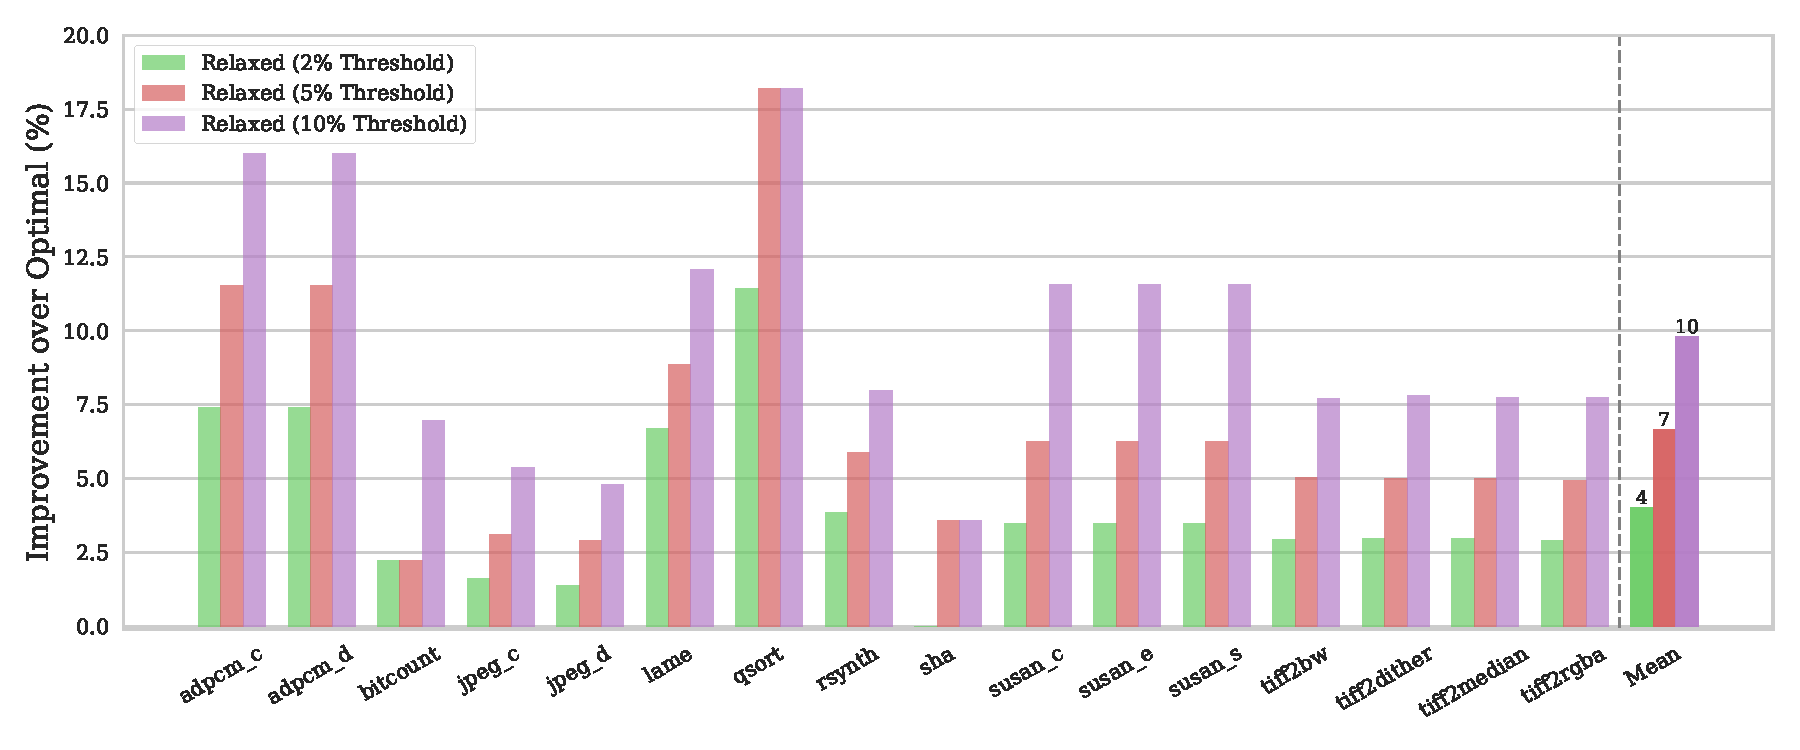
\includegraphics[width=\textwidth]{figs/num-probes-improvement.pdf}
    \caption{Percentage of instrumented basic blocks for the optimal and the relaxed instrumentation with different relaxation thresholds.}
    \label{fig:num-probes-improvement}
\end{figure}

The static errors presented in Figure~\ref{fig:static-instr-error} indicate the amount of error expected by the relaxation algorithm after reducing the number of probes.
This figure shows both the maximum (bars with light colours) and the average (bars with dark colours) static errors observed when relaxing the instrumentation for each DAG of the benchmarks.
Notice that, in most cases, the average static errors are considerably lower than the relaxation threshold, while the maximum static errors are usually close to the threshold.
The average static error shows that in a significant number of DAGs, the relaxation was notably conservative.
This conservatism will be specially evident in the dynamic evaluation.

\begin{figure}[ht]
    \centering
    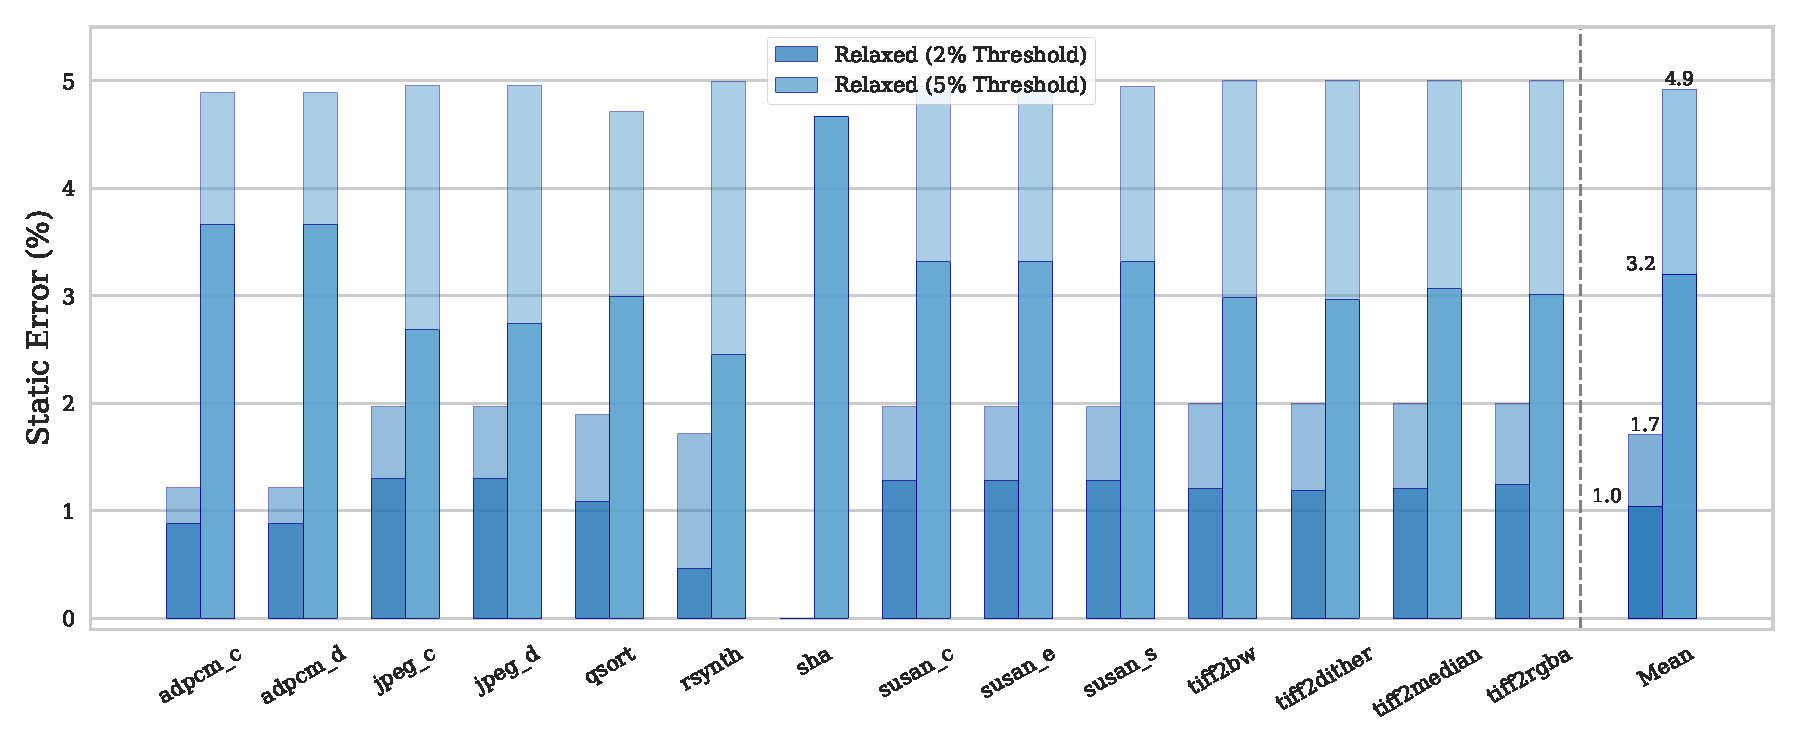
\includegraphics[width=\textwidth]{figs/instr-error.pdf}
    \caption{Average and maximum static error expected for the work profiling, after relaxing the number of probes.}
    \label{fig:static-instr-error}
\end{figure}

\subsection{Dynamic Evaluation}

For the evaluation of the performance overhead that the instrumentation incur to the benchmarks, we measure the wall-clock time of the benchmarks when compiled with the default \texttt{-O3} optimisation.
For each benchmark, we compute the average overhead over all its 1000 input dataset.
When measuring the wall-clock time for each input, in order to reduce noise, we execute the same input until we have a statistically sound measurement, i.e. we execute until we have an interval no larger than 1\% with 99\% confidence.
Figure~\ref{fig:overhead-O3} shows the performance overhead imposed by the work instrumentation on the benchmarks when compared to their non-instrumented counterparts.
Figure~\ref{fig:overhead-improvement-O3} shows the improvement of the relaxation algorithm over the optimial instrumentation, regarding the reduction in overhead.

\begin{figure}[ht]
    \centering
    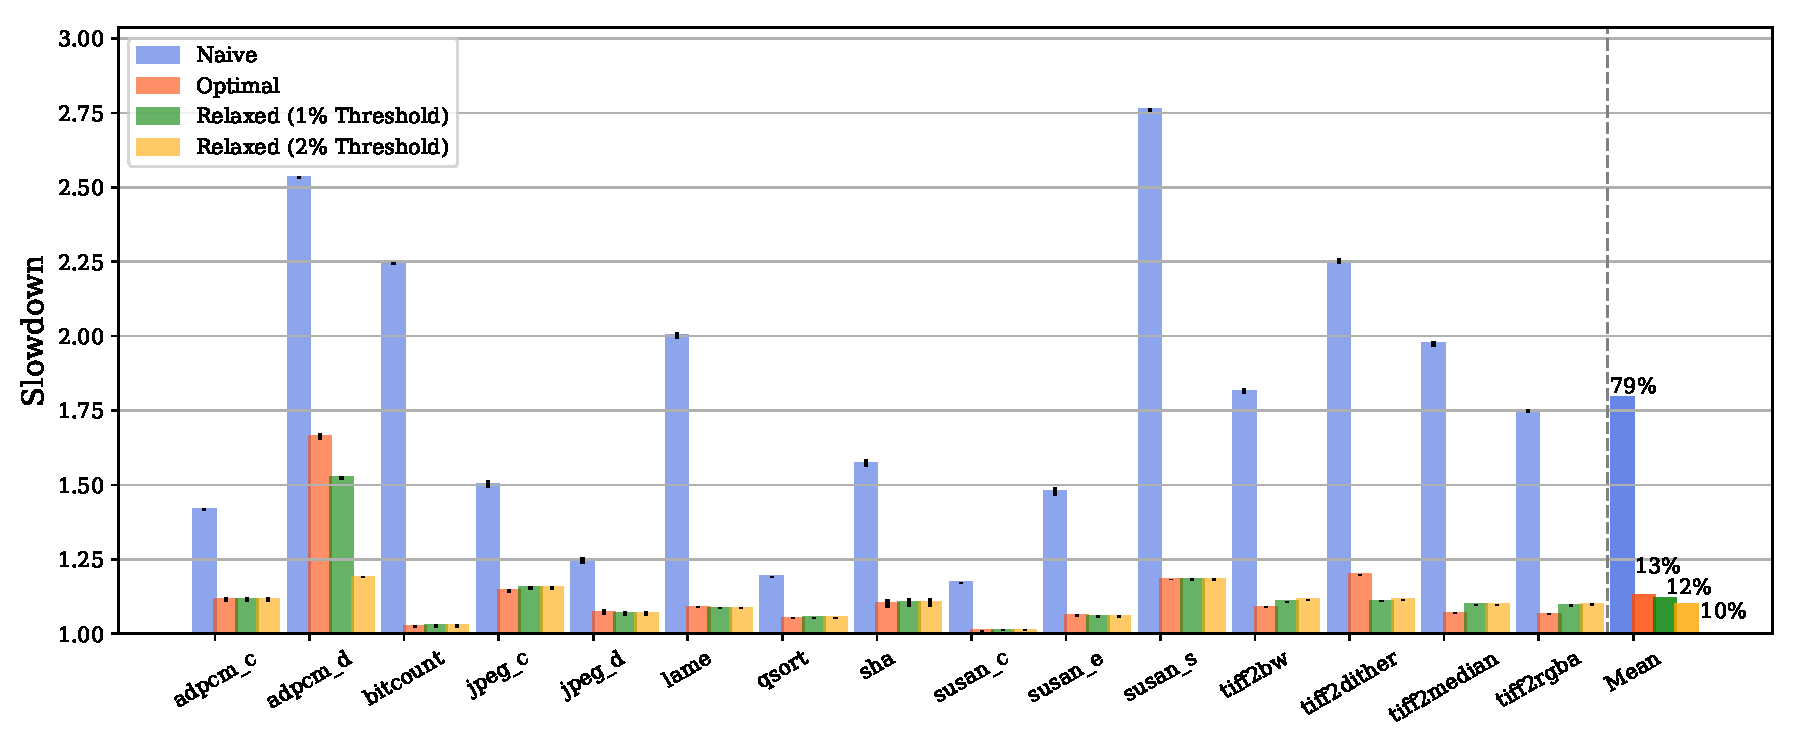
\includegraphics[width=\textwidth]{figs/overhead-O3.pdf}
    \caption{Overhead of the instrumentations compiled with {\texttt{-O3}}.}
    \label{fig:overhead-O3}
\end{figure}

\begin{figure}[ht]
    \centering
    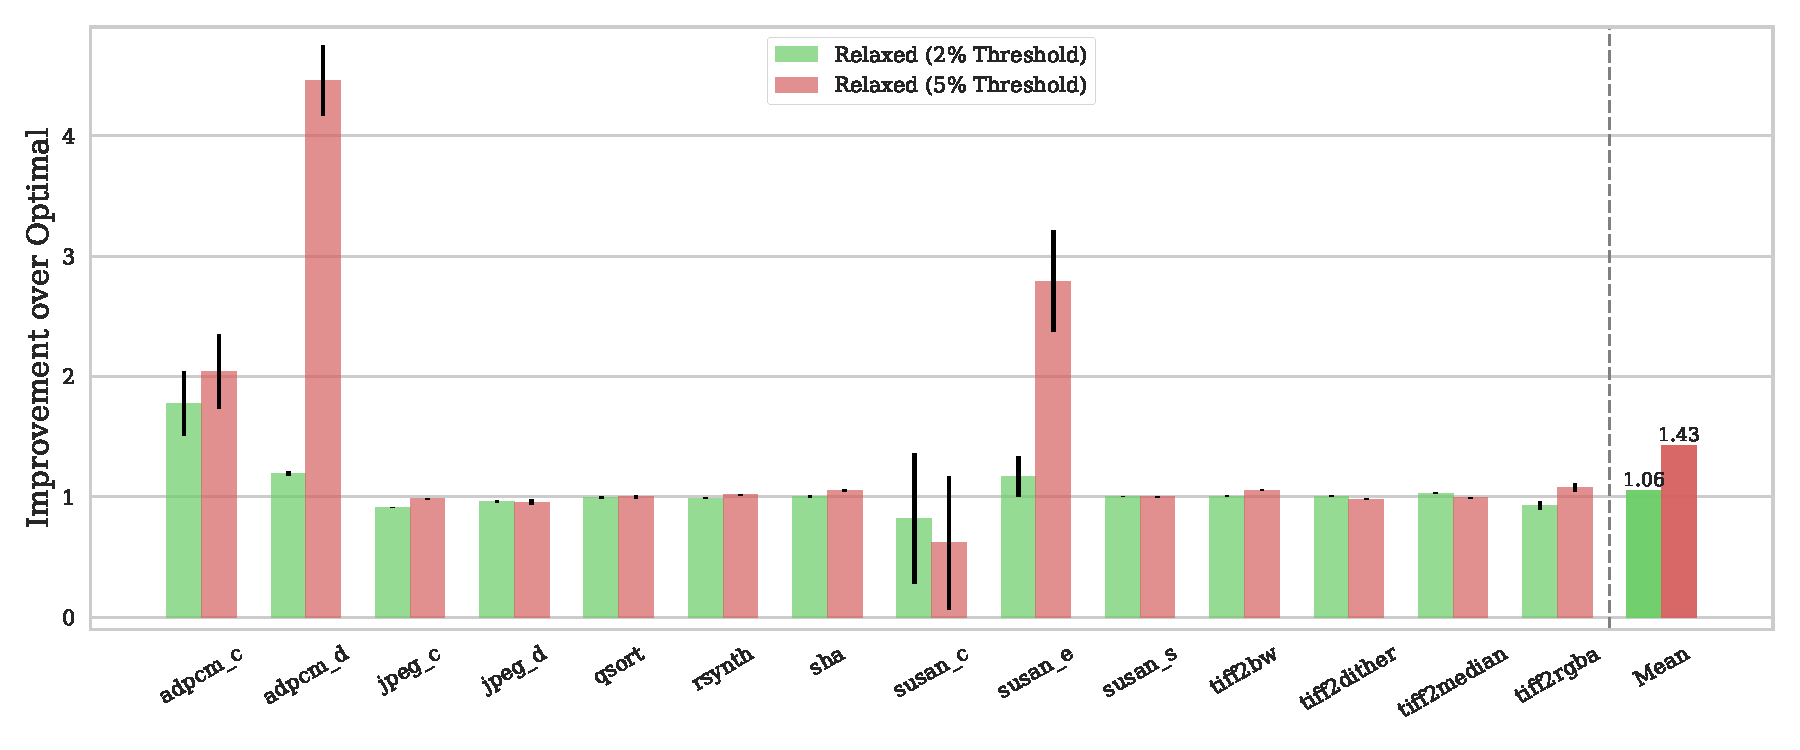
\includegraphics[width=\textwidth]{figs/overhead-improvement-O3.pdf}
    \caption{Overhead of the instrumentations compiled with {\texttt{-O3}}.}
    \label{fig:overhead-improvement-O3}
\end{figure}

Figure~\ref{fig:overhead-improvement-O3} shows that the relaxation algorithm, with 5\% threshold, is able to improve an average of 48\% over the optimal instrumentation, improving about $4.5\times$ for both the \texttt{adpcm\_d} and \texttt{susan\_e} benchmarks.
%If we disconsider the exceptional improvement for the \texttt{adpcm\_d} benchmark, the relaxation algorithm with a 5\% threshold is able to improve an average of about 20\% over the optimal instrumentation.

\textbf{Profile-guided Instrumentation.}

%\textbf{Code size.}
%\begin{figure}[ht]
%    \centering
%    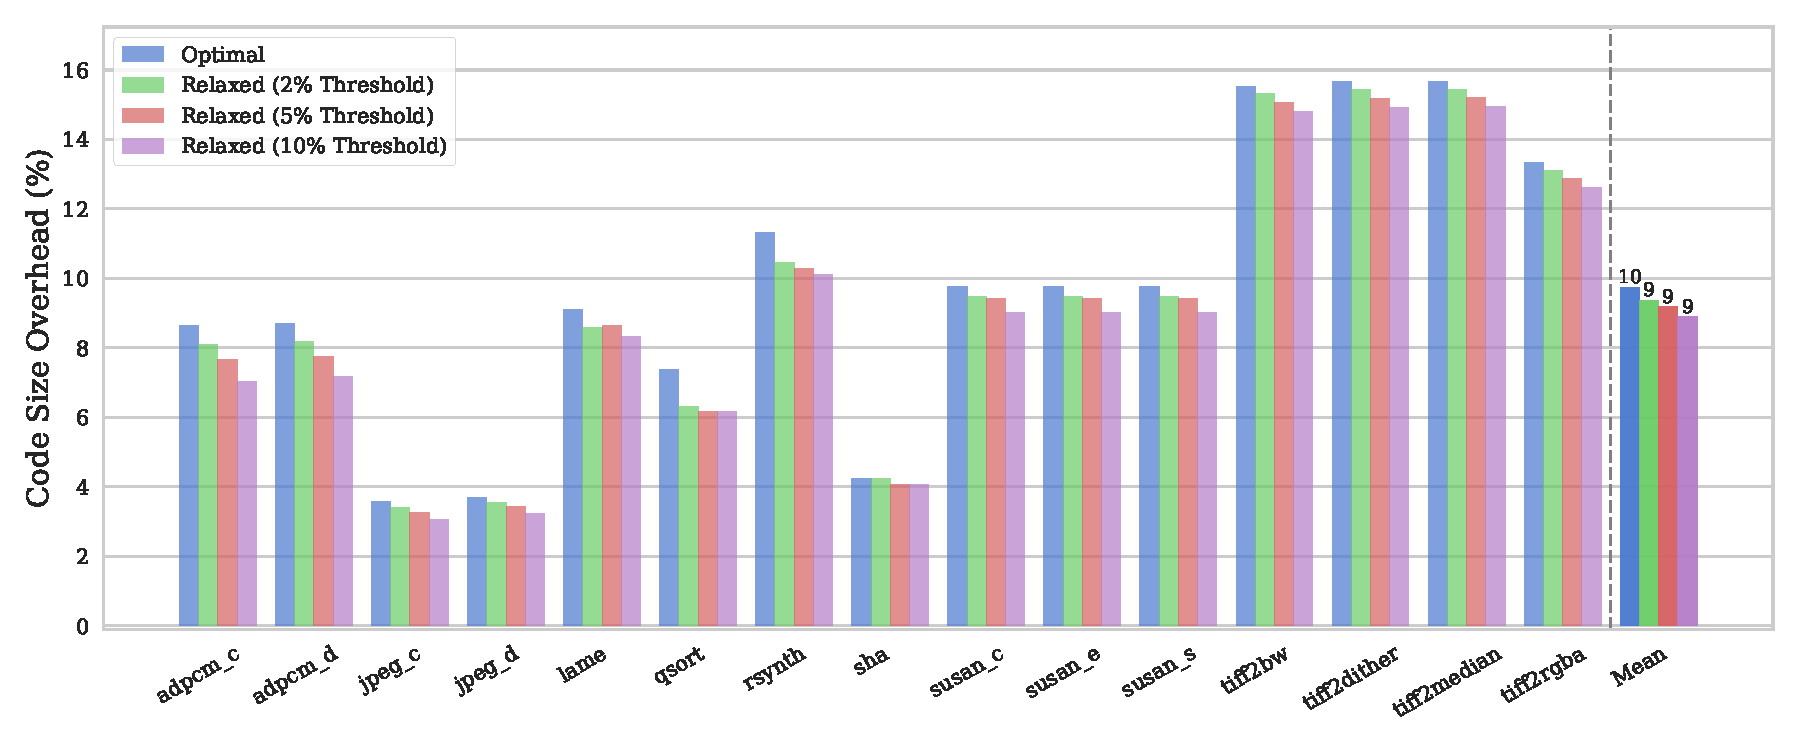
\includegraphics[width=\textwidth]{figs/code-size-probes.pdf}
%    \caption{Percentage of instrumented basic blocks for the optimal and the relaxed instrumentation with different relaxation thresholds.}
%    \label{fig:num-probes}
%\end{figure}
%
%\begin{figure}[ht]
%    \centering
%    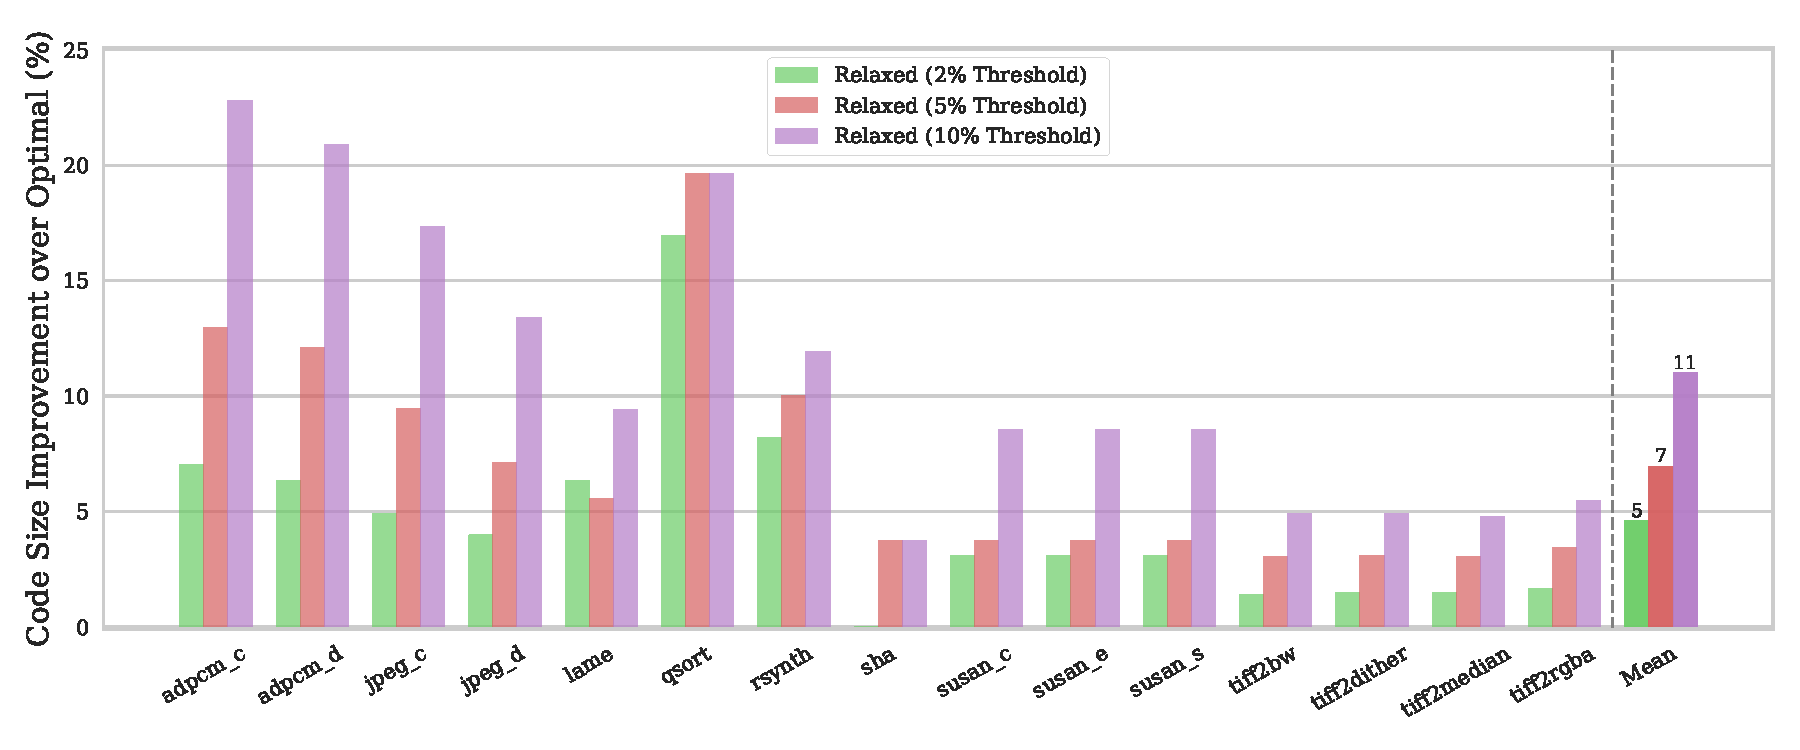
\includegraphics[width=\textwidth]{figs/code-size-probes-improvement.pdf}
%    \caption{Percentage of instrumented basic blocks for the optimal and the relaxed instrumentation with different relaxation thresholds.}
%    \label{fig:num-probes-improvement}
%\end{figure}


%In this section we discuss the three baseline implementations that will be used for assessing the quality of the proposed metric.

%\vspace{1ex}
%\noindent \textbf{{\Itercomp} over a single input}

%Most of the existing {\itercomp} studies find the best optimisation though repeated runs on the same input.
%Although this approach will usually lead to sub-optimal performance across large input datasets, it provides a good baseline when considering the complexity and resonably low compile-time regarding iterative optimising compilers.
%If $M$ is the total number of combinations of compiler optimisations, this approach requires $O(M)$ runs of the program being optimised.
%We can consider two main scenarios:
%\textit{($i$ - best case scenario)} after selecting the optimisation over each individual input, consider the one with best performance across the whole input dataset;
%\textit{($ii$ - expected scenario)} after selecting the optimisation over each individual input, consider the average case of their performance across the whole input dataset.

%\vspace{1ex}
%\noindent \textbf{{\Itercomp} across large input datasets}

%Recent work on {\itercomp} have been targeting optimisation across multiple inputs~\cite{fursin07,chen10,chen12a}.
%If $N$ is the number of input test cases and $M$ is the total number of combinations of compiler optimisations, they perform a total of $O(NM)$ runs of the program being optimised.
%Similarly to what have been discussed previously, there are different ways for how to determine the optimal combination of compiler optimisations across multiple inputs.
%It is possible to tune the selection of the program-optimal combination to minimise risk or to maximise average performance.
%A compromise-based selection criterion could be to maximise average speedup with minimised variance.

\subsection{Case Studies}

\noindent \textbf{Analysis of the Best Improvement in Overhead: \texttt{adpcm\_d}}

The \texttt{adpcm\_d} benchmark is the most critical case amongst the evaluated benchmarks, with an overhead of about 59\% for the optimal instrumentation.
This benchmark consists mainly of a single hot loop with several branches inside it, as depicted by Figure~\ref{fig:adpcm_d-cfg-instr}.
The relaxation algorithm is able to reduce this overhead down to about 47\% (with a static error threshold of 2\%) and 14\% (with a static error threshold of 5\%) by removing only one and two probes from the hot loop, respectively.
These overhead reductions represent a 20\% and 4.5$\times$ improvement over the optimal algorithm, with 2\% and 5\% relaxation threshold respectively.
The two relaxed probes were placed in branches, inside the hot loop, with a high probability of being taken, but with a small contribution to the total amount of work measured in the loop.

\begin{figure*}[htb]
    \centering
    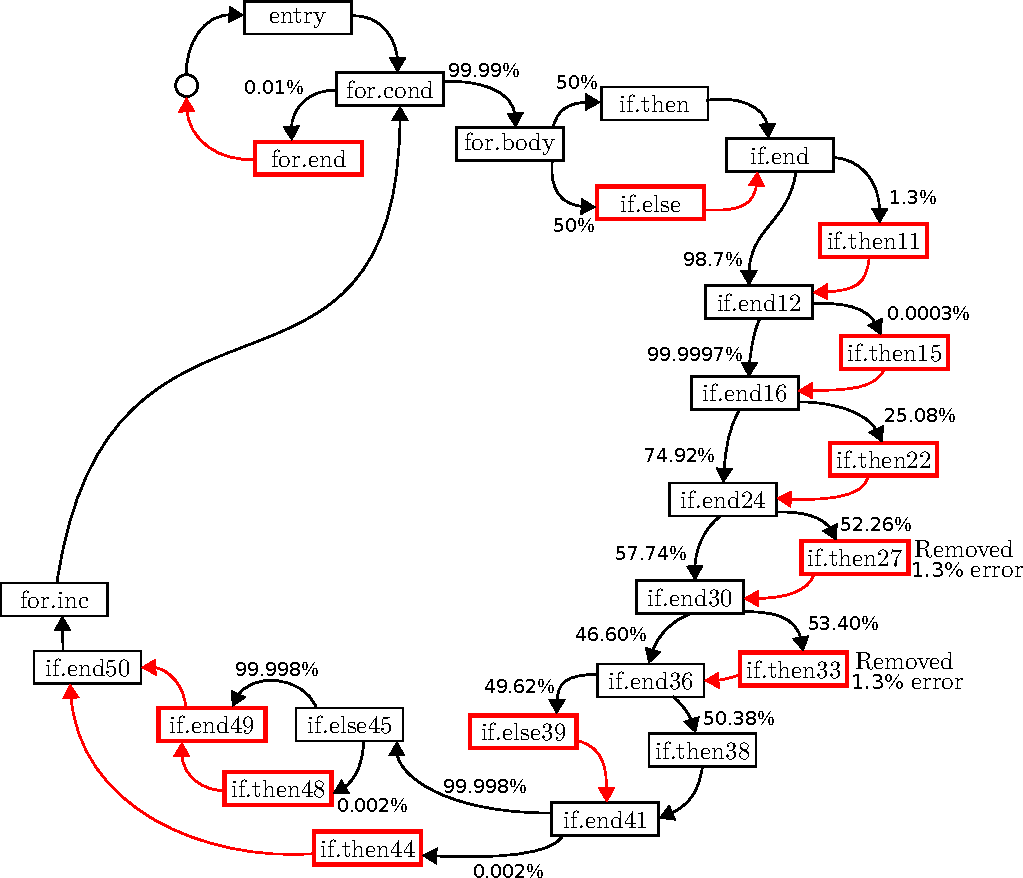
\includegraphics[width=0.8\textwidth]{figs/adpcm_d-cfg-instr.pdf}
    \caption{CFG of the function that contains the hot loop of the \texttt{adpcm\_d} benchmark.}
    \label{fig:adpcm_d-cfg-instr}
\end{figure*}

Figure~\ref{fig:adpcm_d-probes-err-freq} shows all the probes necessary for the function that contains the hot loop of the \texttt{adpcm\_d} benchmark.
Notice that the relaxation was able to remove all probes with an static error lower than the 5\% threshold.
Because these probes were placed in basic blocks with a considerable execution frequency, their removal resulted in a significant reduction in performance overhead.

\begin{figure*}[htb]
    \centering
    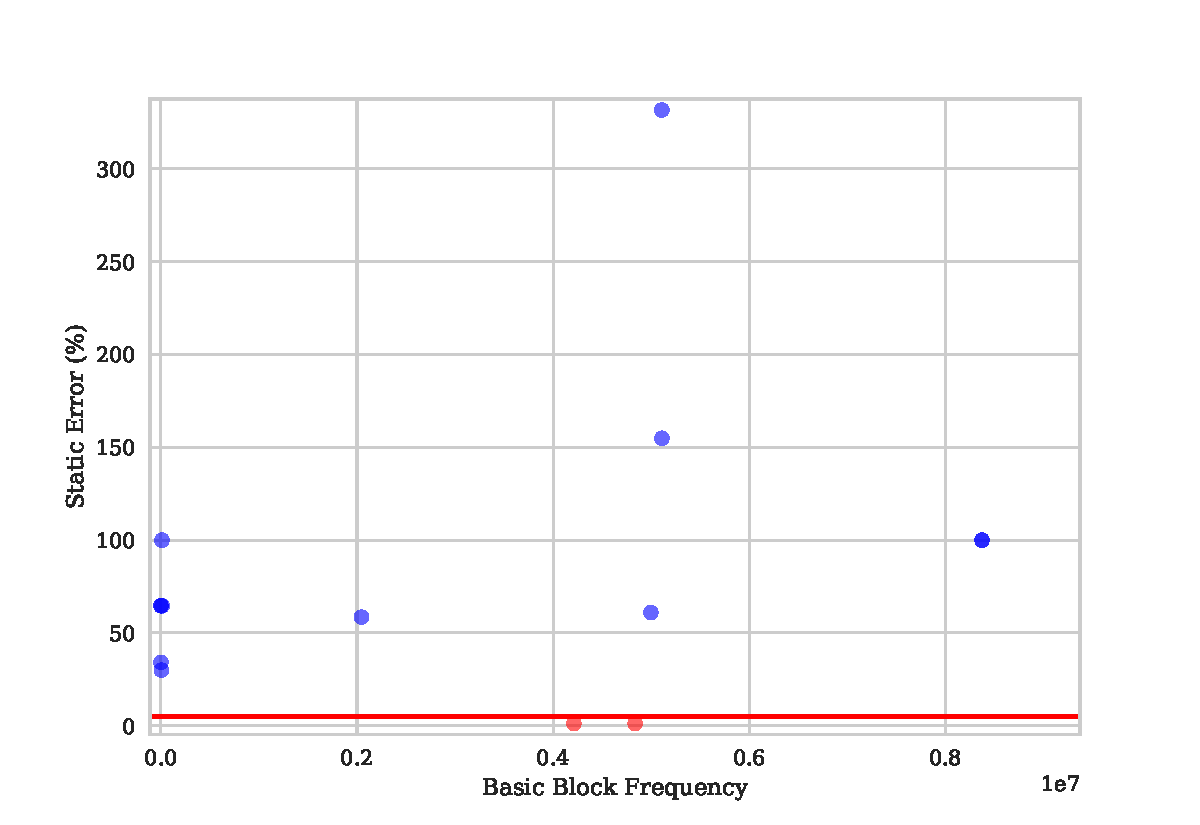
\includegraphics[width=0.8\textwidth]{figs/adpcm_d.pdf}
    \caption{Comparison between probe frequency and static error for the \texttt{adpcm\_d} benchmark. The red line marks the 5\% threshold limit.}
    \label{fig:adpcm_d-probes-err-freq}
\end{figure*}


\noindent \textbf{Analysis of the Abnormal Regression: \texttt{susan\_c}}

\begin{figure*}[htb]
    \centering
    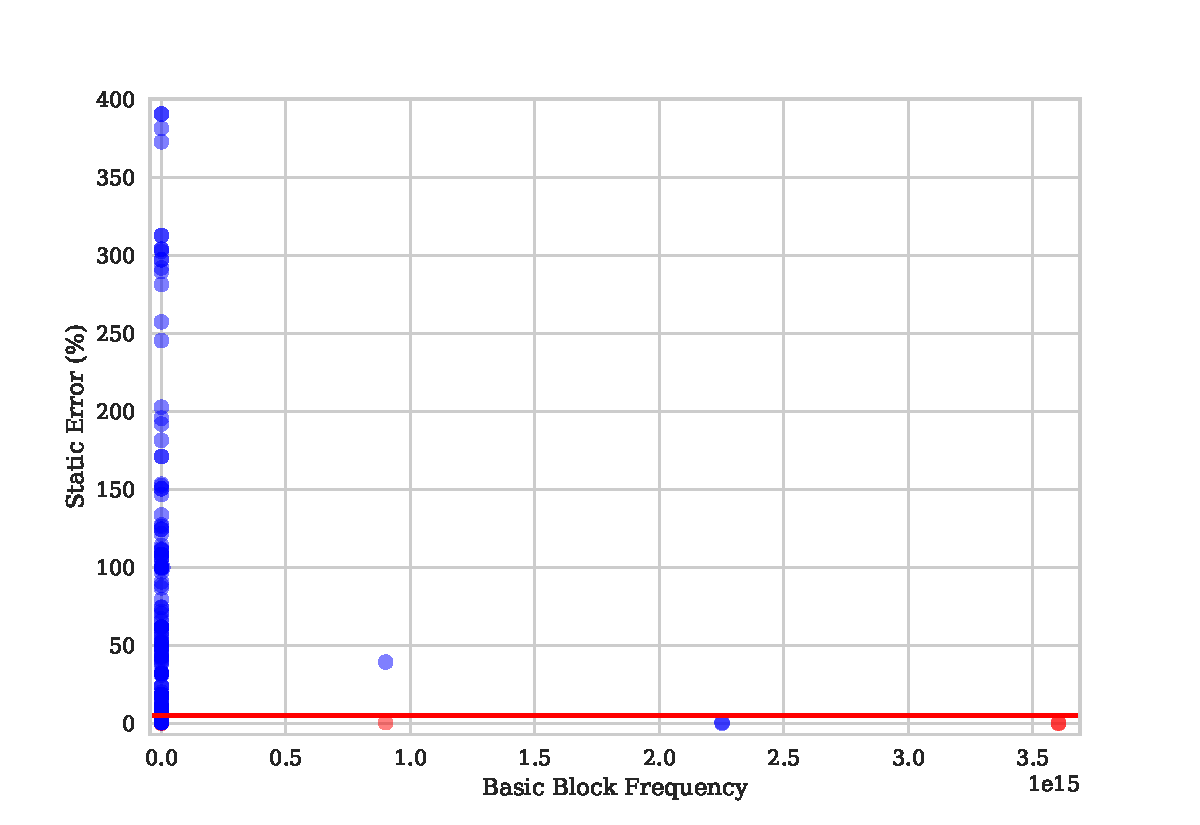
\includegraphics[width=0.8\textwidth]{figs/susan_c.pdf}
    \caption{Comparison between probe frequency and static error for the \texttt{susan\_c} benchmark. The red line marks the 5\% threshold limit.}
    \label{fig:speedups}
\end{figure*}


%\vspace{1ex}
%\noindent \textbf{{\Itercomp} based on the IPC metric}

%While the previous two baselines addresses two opposite aspects of {\itercomp}, namely, compile-time efficiency and performance of the generated code, we also intend to compare against IPC as the competing baseline.
%The main reason for comparing against IPC is because it has been proposed as a metric for comparing the performance of two optimisations running on two distinct inputs.
%If $M$ is the total number of combinations of compiler optimisations, this approach requires $O(M)$ runs of the program being optimised.

\section{Evaluation of the Online {\IterComp}}

In this section we evaluate the online {\itercomp} guided by the work-based performance metric.
For comparison, we use the following baselines and configurations:
\begin{itemize}
\item \textbf{Oracle-RM} executes the program multiple times for each input, measuring the real speedup for each compiler optimisation, and then uses the real speedup over \texttt{-O0} for comparing the optimisations.
The speedups are computed based on the wall-clock time.
In order to reduce noise, the program is executed several times for the same input, until the confidence interval no larger than 1\% for a 99\% confidence.
\item \textbf{Oracle-PP} represents an oracle with a \textit{perfect} non-intrusive profiling.
Although it uses the work-based performance metric for comparing optimisation, this oracle also avoids noise in its measurements by also executing the program multiple times for each input.
The first execution is used for profiling the work metric.
The remaining executes are used for measuring the wall-clock time without using the work profiling.
\item \textbf{Real-OP} corresponds to the online {\itercomp} as it would be applied in a real online scenario.
      For each optimisation, a random sample of input is selected, and the program is executed only once with each input.
      The average of the work-based performance metric, $\frac{\Delta W}{\Delta t}$, for the sample of input is then used for selecting the best optimisation.
\item \textbf{Real-R5}
\end{itemize}
In all configurations, the same optimisation is used for multiple distinct inputs, using a dynamic window size, as explained in Section~\ref{sec:oic-infra}.
This window size provides an estimate for the optimisation performance across inputs.
When selecting the best optimisation, they are ranked by the average of their performance measurement, using the work-based performance metric, except for the Oracle-RM which uses the real speedup over \texttt{-O0}.
Figure~\ref{} shows the average window size for each benchmark and configuration.

\begin{figure*}[htb]
    \centering
    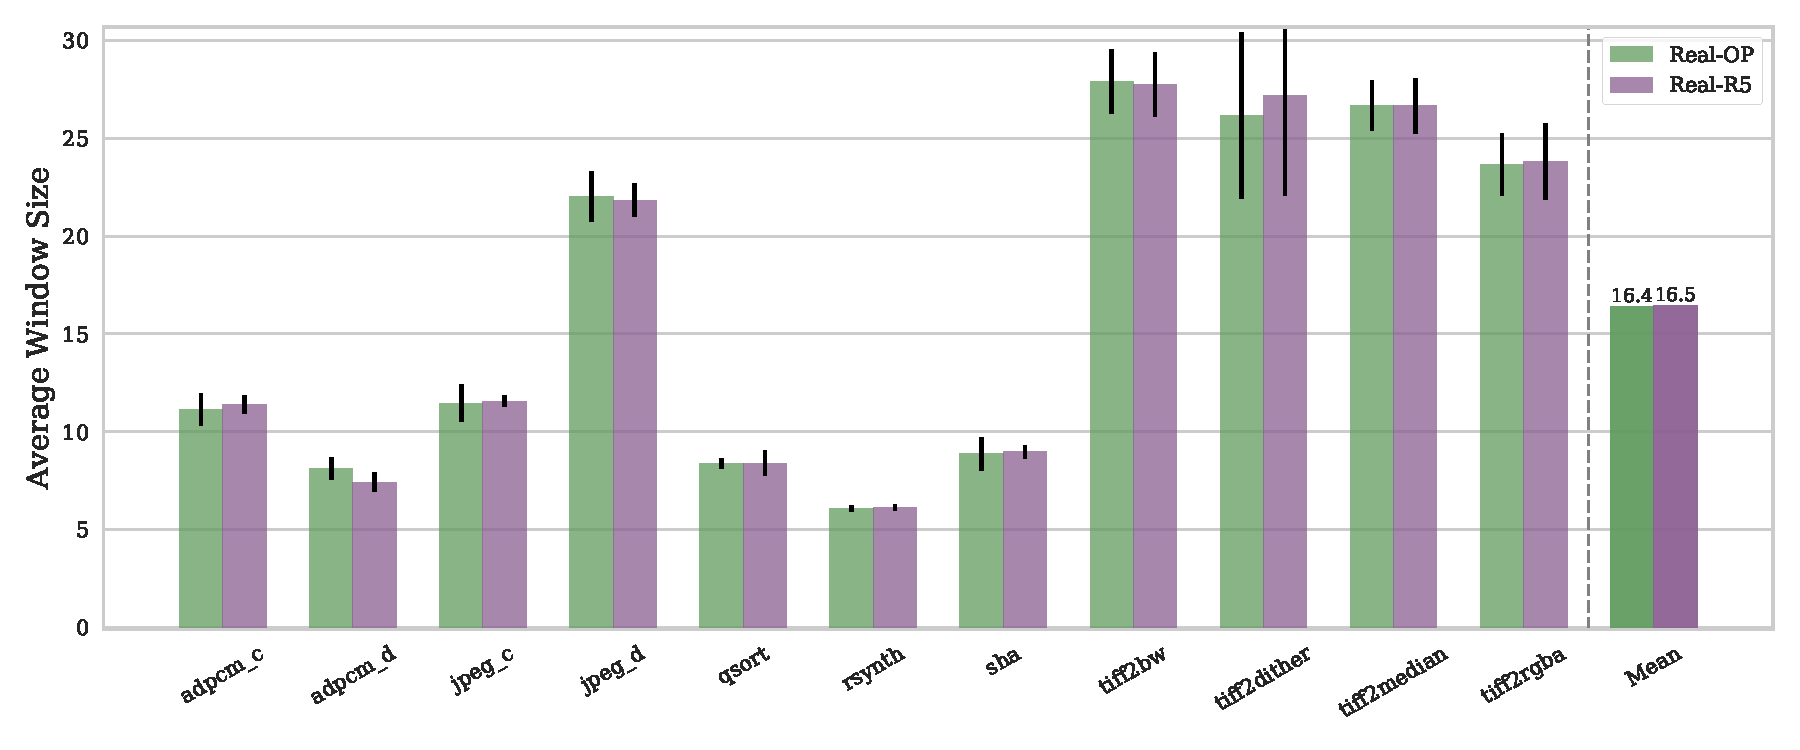
\includegraphics[width=\textwidth]{figs/window-size.pdf}
    \caption{Average window size observed during the online {\itercomp}.}
    \label{fig:speedups}
\end{figure*}

For the purpose of evaluating the use of the work-based performance metric for guiding the optimisation search, we collected in advance a fixed set of optimisations.
This set contains 500 optimisations collected in a random search using the training benchmarks.
These optimisations contain an average of 40 passes, including repetitions, with a maximum of 119 optimisation passes and minimum, but it also contains optimisations which consists of a single flag, such as the default optimisations \texttt{-O1}, \texttt{-O2}, \texttt{-O3}, \texttt{-Os}, and \texttt{-Oz}.

  \begin{minipage}{0.9\textwidth}
     \vspace{1em}
     \singlespace
     \noindent\textbf{Example of a long optimisation sequence:}\vspace{-1ex}
     \justify{\usefont{T1}{cmr}{m}{n} -globalopt -reassociate -instcombine -loop-rotate -block-freq -deadargelim -early-cse -sroa -argpromotion -sccp -tbaa -barrier -constmerge \mbox{-loop-vectorize} -domtree -basicaa -memdep -basiccg -memcpyopt \mbox{-constprop} -adce -globaldce -mem2reg -constmerge \mbox{-globaldce} -constprop -instsimplify -dse -dce -simplifycfg -loop-unroll -reassociate -constprop \mbox{-globaldce} -instsimplify -adce -constmerge -bb-vectorize -dce -mergefunc -simplifycfg -dse -loop-unroll -globaldce}
  \end{minipage}

  \begin{minipage}{0.9\textwidth}
     \vspace{1em}
     \singlespace
     \noindent\textbf{Example of a short optimisation sequence:}\vspace{-1ex}
     \justify{\usefont{T1}{cmr}{m}{n} -mem2reg -simplifycfg -constprop -dce}
  \end{minipage}

  \begin{minipage}{0.9\textwidth}
     \vspace{1em}
     \singlespace
     \noindent\textbf{Example of an optimisation sequence which includes {-O3}:}\vspace{-1ex}
     \justify{\usefont{T1}{cmr}{m}{n} -O3 -adce -globaldce -simplifycfg -memcpyopt -reassociate -mergefunc \mbox{-dce} -dse}
     \vspace{2em}
  \end{minipage}

In order to evaluate the quality of the final optimisation selected by the {\itercomp} search, we compare their speedup by measuring wall-clock time of the benchmarks when compiled with the default \texttt{-O3} optimisation.
For each benchmark, after selecting the final optimisation, we compute the average speedup over all the 1000 input dataset.
When measuring the wall-clock time for each input, in order to reduce noise, we execute the same input until we have a statistically sound measurement, i.e. we execute until we have an interval no larger than 1\% with 99\% confidence.
Figure~\ref{fig:speedups-per-input} shows the histogram of the speedups obtained for each benchmark with all their respective 1000 inputs.
This figure shows the speedups of the best optimisation found by the oracle with real measurements of execution time (Oracle-RM).
It illustrates the expected upper bound by the online {\itercomp}.


\begin{figure*}[htb]
    \centering
    %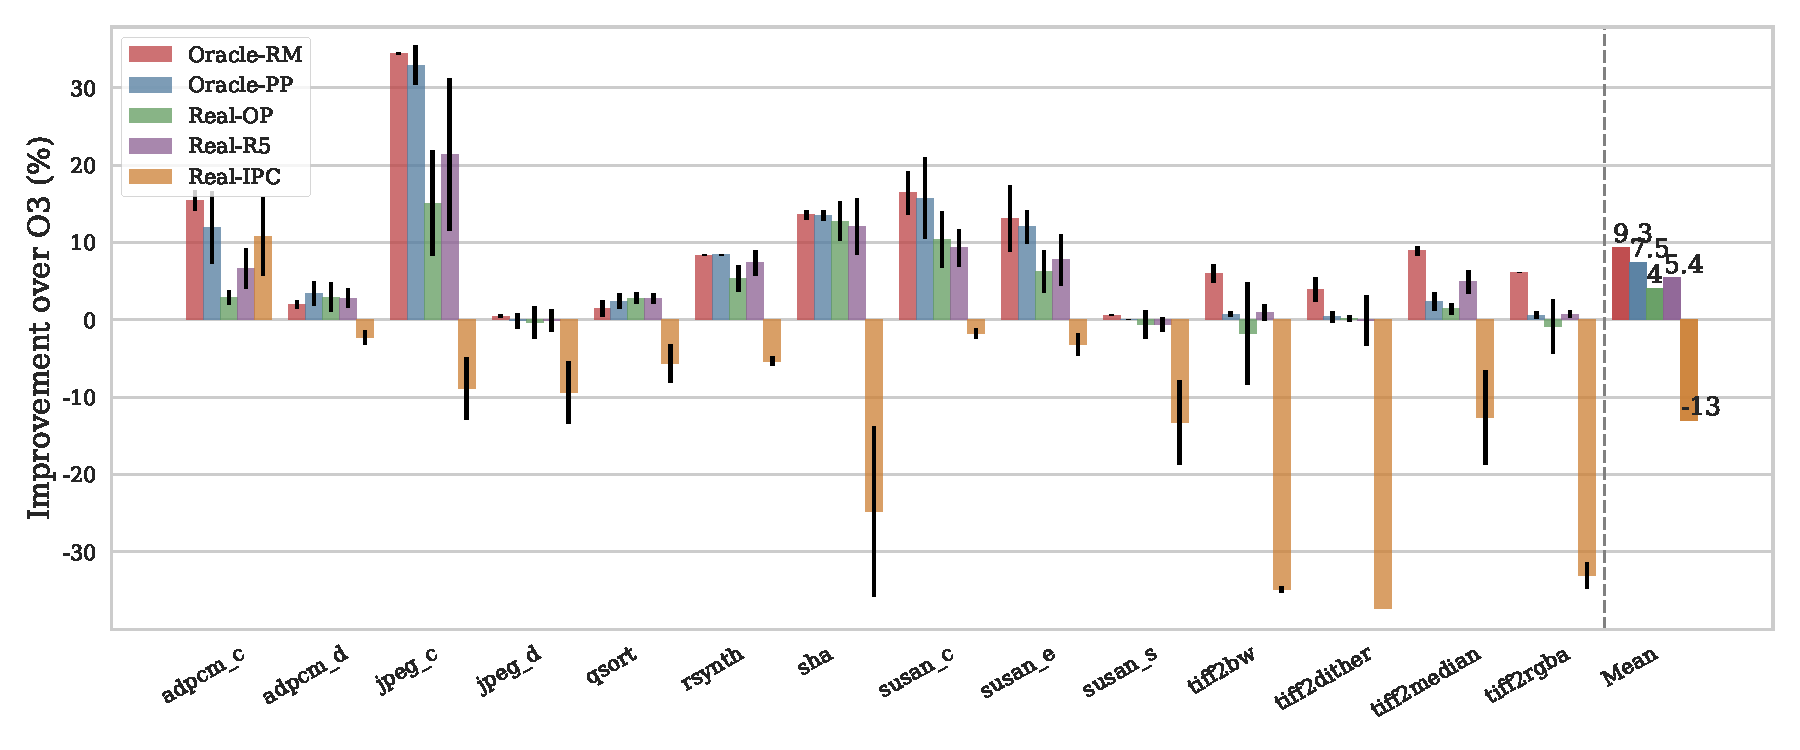
\includegraphics[width=\textwidth]{figs/speedups.pdf}
    \caption{Speedups obtained from the final optimisation selected by the online {\itercomp}.
	         The speedups reported for each benchmark represents the average speedup across their complete 1000 input datasets.}
    \label{fig:speedups}
\end{figure*}
 
Figure~\ref{fig:speedups-per-input} is also important for showing that, although some of the benchmarks have a very consistent speedup for all their inputs,
other benchmarks are highly sensitive to the input.
For example, the optimisation with best average performance for the \texttt{adpcm\_d} benchmark presents a wide range of speedups across all its inputs,
varying from 0.7 up to about 1.5 of speedup.
On the other hand, although the best optimisation selected for the \texttt{jpeg\_d} benchmark has a much shorter range of speedups, there is a clear concentration of inputs around two different speedups.
These results corroborate the claim that performing {\itercomp} on a single input can be misleading and cause the optimisation search to overfit.

\begin{figure}[h!]
    \centering
    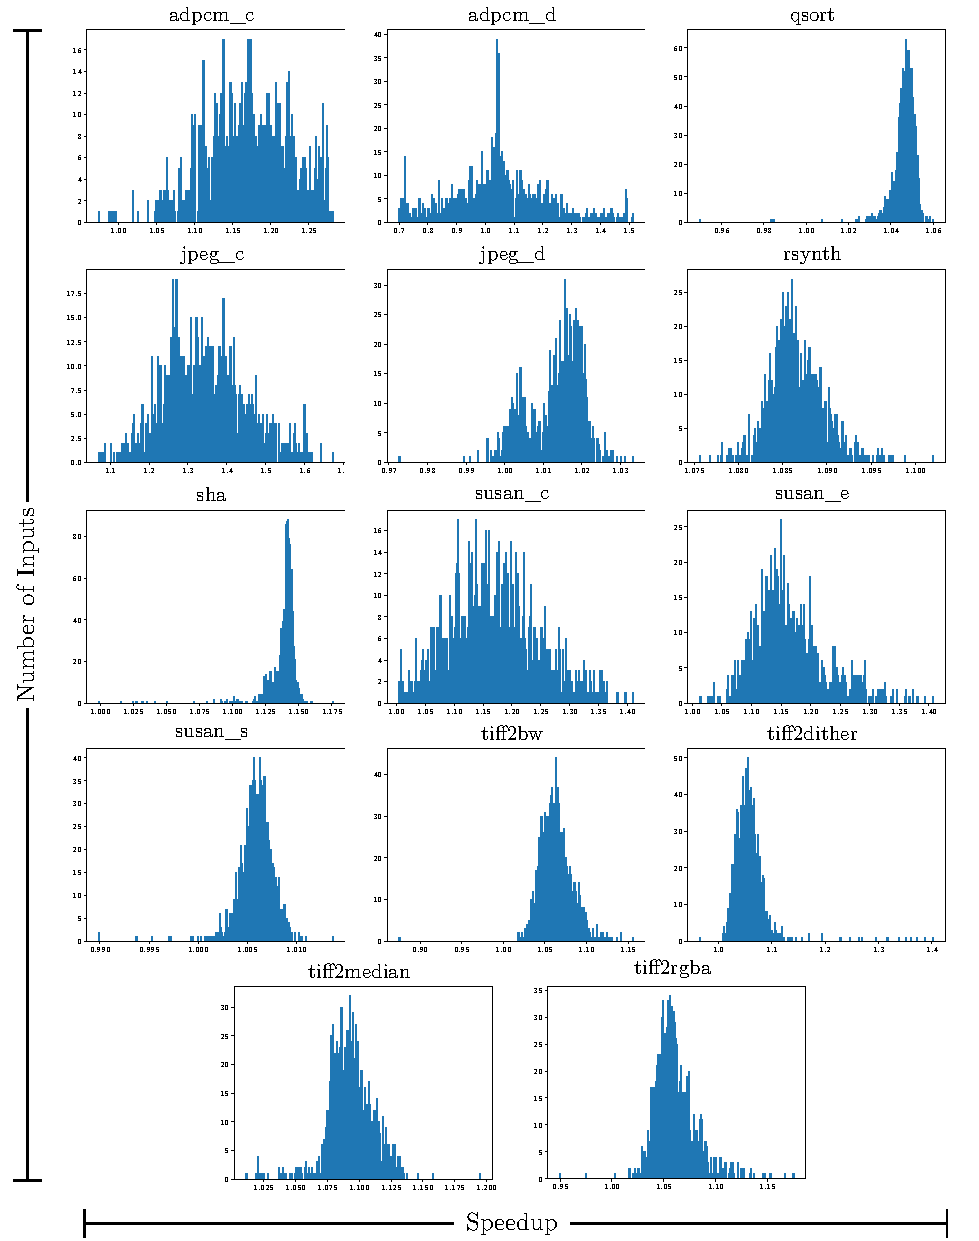
\includegraphics[width=\textwidth]{figs/speedups-per-input.pdf}
    \caption{Histograms for the speedups over \texttt{-O3} with the complete dataset of 1000 inputs for each benchmark.
             In each case, we are using the optimisation with the best average speedup over \texttt{-O3}.
             This figure shows how the performance for some of the benchmarks are highly sensitive to the input.}
    \label{fig:speedups-per-input}
\end{figure}

%\begin{figure*}[htb]
%    \centering
%    \includegraphics[width=\textwidth]{figs/profiled-speedups.pdf}
%    \caption{Speedups observed with the online {\itercomp} if we
%             consider the instrumentation overhead.}
%    \label{fig:profiled-speedups}
%\end{figure*}

\subsection{Contribution of individual optimisation passes}

Figure~\ref{fig:flagsfreq} shows an aggregated view of the final combination of compiler optimisations that were selected by {\itercomp} search.
The figure presents the individual optimisation passes with at least 1\% of frequency in the selected combination of compiler optimisations that improved the performance over {\texttt{-O3}}.

\begin{figure*}[htb]
    \centering
    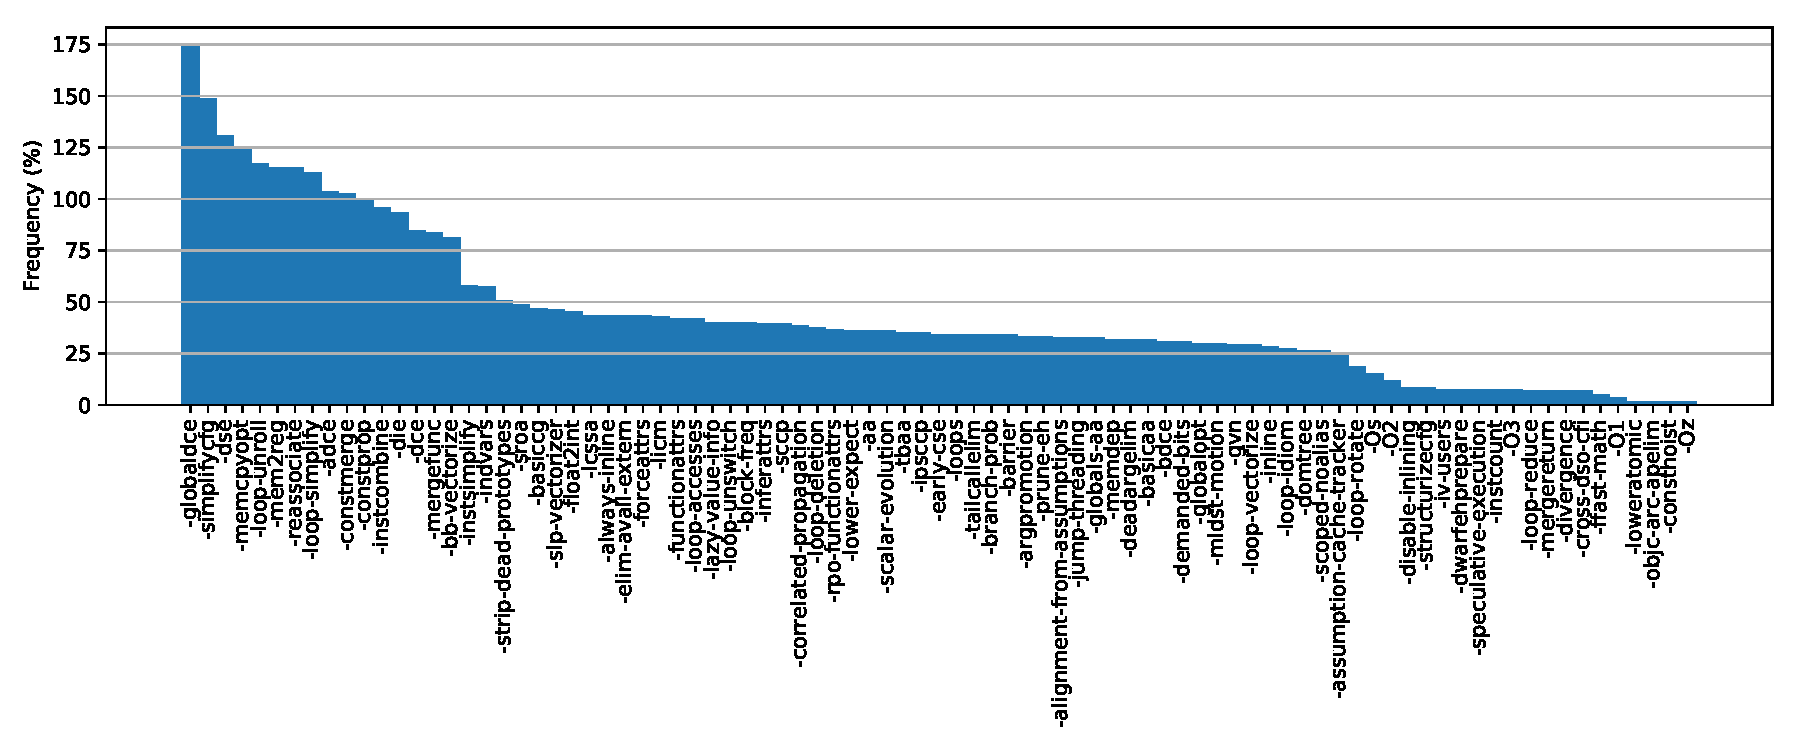
\includegraphics[width=\textwidth]{figs/flagsfreq.pdf}
    \caption{Frequency of individual optimisation passes on the final selected 
             compiler optimisations of the {\itercomp} search over
             all benchmarks.}
    \label{fig:flagsfreq}
\end{figure*}

\subsubsection{Inter-Procedural Optimisations}
%\begin{description}
\noindent\textbf{Dead Global Elimination (\texttt{-globaldce}):}
It is an inter-procedural optimisation that eliminates unreachable internal globals from the program.
It uses an aggressive algorithm that searches for global definitions that are known to be alive.
After finding all live global definitions, it deletes all remaining globals.
%This allows it to delete recursive chunks of the program which are unreachable.

\noindent\textbf{Merge Functions \texttt{-mergefunc}:}
This pass looks for equivalent functions that are mergable and folds them.
It introduces a function encoding which allows it to provide a total-ordering for the function set.
The total-ordering allows to arrange functions into the binary tree.
When iterating over the functions, it checks for an equivalent function in tree.
If an equivalent function exists, both functions are merged, otherwise, the new function is added to the tree.
This pass focus mainly on improving code size and memory footprint.
%The lookup routine has $O(log(n))$ complexity, while the whole merging process has complexity of $O(n\cdot log(n))$.

\subsubsection{Transformations of the CFG}

\noindent\textbf{Simplify the CFG \texttt{-simplifycfg}:}
This optimisation simplifies the CFG by basic blocks merging and dead code elimination, such as:
eliminates a basic block that only contains an unconditional branch;
removes basic blocks with no predecessors;
eliminates PHI nodes for basic blocks with a single predecessor; etc.
This pass makes use of LLVM's built-in cost model to decide when it is beneficial for performing such transformations.

\noindent\textbf{Canonicalize Natural Loops \texttt{-loop-simplify}:}
This pass performs several transformations to convert natural loops into a simpler form, which makes subsequent analyses and transformations simpler and more effective.
Loop pre-header insertion guarantees that there is a single, non-critical entry edge from outside of the loop to the loop header.
This simplifies a number of analyses and transformations, such as Loop Invariant Code Motion (LICM).
Loop exit-block insertion guarantees that all exit blocks from the loop (blocks which are outside of the loop that have predecessors inside of the loop) only have predecessors from inside of the loop (and are thus dominated by the loop header). This simplifies transformations such as store-sinking that are built into LICM.
This pass also guarantees that loops will have exactly one backedge.
Note that the \texttt{-simplifycfg} pass will clean up blocks which are split out but end up being unnecessary, so usage of this pass should not pessimize generated code.

\noindent\textbf{Unroll Loops \texttt{-loop-unroll}:}
This pass implements a simple loop unroller.
It works best when loops have been canonicalized by the \texttt{-indvars} pass, allowing it to determine the trip counts of loops easily.
This pass makes use of LLVM's built-in cost model to estimate the computational cost of both rolled and unrolled loops, which enables it to perform loop unrolling only when it is profitable.

\subsubsection{Dead Code Elimination}

\noindent\textbf{Dead Instruction Elimination \texttt{-die}:}
Dead instruction elimination performs a single pass over the function, removing instructions that are obviously dead.

\noindent\textbf{Dead Store Elimination \texttt{-dse}:}
A trivial dead store elimination that only considers basic-block local redundant stores.

\noindent\textbf{Dead Code Elimination \texttt{-dce}:}
Dead code elimination is similar to dead instruction elimination, but it rechecks instructions that were used by removed instructions to see if they are newly dead.
In other words, it performs dead instruction elimination until it reaches a fixed point.

\noindent\textbf{Aggressive Dead Code Elimination \texttt{-adce}:}
ADCE aggressively tries to eliminate code.
This pass is similar to DCE but it assumes that values are dead until proven otherwise.
This is similar to SCCP, except applied to the liveness of values.

\subsubsection{Simplification of Expressions}

\noindent\textbf{Combine redundant instructions \texttt{-instcombine}:}
Combine instructions to form fewer, simple instructions, by means of algebraic simplifications.
This is a simple worklist driven algorithm, in a peephole fashion.
Some of the simplifications and canonicalizations are:
Constant operands are moved to the right-hand side of commutative binary operations;
Multiplications with a constant power-of-two argument are transformed into shifts;
All compare instructions on boolean values are replaced with logical operations.
This pass can also simplify calls to specific well-known function calls (e.g. runtime library functions).
For example, a call exit(3) that occurs within the main() function can be transformed into simply return 3.

\noindent\textbf{Reassociate expressions \texttt{-reassociate}:}
This pass reassociates commutative expressions in an order that is designed to promote better constant propagation, Global Common Subexpression Elimination (GCSE), LICM, etc.
It performs a canonical reordering of the operands of commutative binary operations.

\noindent\textbf{Merge Duplicate Global Constants \texttt{-constmerge}:}
Merges duplicate global constants together into a single constant that is shared. This is useful because some passes (i.e., TraceValues) insert a lot of string constants into the program, regardless of whether or not an existing string is available.

\noindent\textbf{Simple constant propagation \texttt{-constprop}:}
This pass implements constant propagation and merging.
It looks for instructions involving only constant operands and replaces them with a constant value instead of an instruction
This pass has a habit of making definitions be dead.
It is a good idea to run a Dead Instruction Elimination pass sometime after running this pass.

\subsubsection{Other Frequent Transformations}

\noindent\textbf{MemCpy Optimization \texttt{-memcpyopt}:}
This pass performs various transformations related to eliminating \texttt{memcpy} calls, or transforming sets of stores into \texttt{memsets}.

\noindent\textbf{Promote Memory to Register \texttt{-mem2reg}:}
This file promotes memory references to be register references. It promotes alloca instructions which only have loads and stores as uses. An alloca is transformed by using dominator frontiers to place phi nodes, then traversing the function in depth-first order to rewrite loads and stores as appropriate. This is just the standard SSA construction algorithm to construct “pruned” SSA form.


\noindent\textbf{Basic-Block Vectorization \texttt{-bb-vectorize}:}
This pass combines instructions inside basic blocks to form vector instructions.
The algorithm was inspired by that used by \cite{franchetti05}.
It iterates over each basic block, attempting to pair compatible instructions, repeating this process until no additional pairs are selected for vectorization.
When the outputs of some pair of compatible instructions are used as inputs by some other pair of compatible instructions, those pairs are part of a potential vectorization chain.
Instruction pairs are only fused into vector instructions when they are part of a chain longer than some threshold length.
Moreover, the pass attempts to find the best possible chain for each pair of compatible instructions.
These heuristics are intended to prevent vectorization in cases where it would not yield a performance increase of the resulting code.



%\end{description}

\section{Summary}

